\section{Online Search}
In the preceeding section we showed that it is possible to break a large 
number of path symmetries by decomposing a 4-connected grid map into 
a set of empty rectangular rooms and pruning all nodes from the interior of
each room.
However, it is often the case that a pruned node might be required at a later
point as a start or goal location for an agent.
To solve this problem we propose to insert the start or goal (or both if necessary)
back into the graph for the duration of the search using the following procedure:
\begin{enumerate}
\item{If the start and goal are not in the same room, connect each of them
to the closest neighbours on each side of the perimeter of the empty room (see Figure \ref{fig-insertion}).}
\item{If the start and goal are in the same room no insertion is required;
 take the manhattan distance between them as the length of the optimal path (see Figure \ref{fig-noinsertion}).}
\end{enumerate}
We claim that this procedure does not affect the optimality guarantees associated with traversing
across the room that the start or goal node is located in. 

\begin{lemma}
Let $R$ be an empty rectangular room and $N \in R$ the set of interior nodes.
Given any optimal length path segment $\pi^*(s, g)$ where $s, g \in R$
it is always possible to construct another optimal length path $\pi'(s, g)$ which 
mentions only the nodes in $\lbrace s, g \rbrace \bigcup  R \setminus N$.
\end{lemma}
\begin{proof}
First, suppose $s \in N$ and $g \in R \setminus N$ (or vice versa).
In this case we insert $s$ into $R \setminus N$ and connect it 
to $\lbrace s'_{1}, s'_{2}, s'_{3}, s'_{4} \rbrace \in R \setminus N$; the closest neighbours on each side of the perimeter.
The weight of each edge incident with $s$ is equal to the manhattan distance between
$s$ and each $s'_{i}$.
Thus both $s, g \in \lbrace s, g \rbrace \bigcup R \setminus N$.
Since $g$ is on the perimeter of $R$, there must exist a path $\pi(s'_{i}, g)$ and
we can now construct $\pi'(s, g)$ as $\pi'(s, g) = \pi(s,s'_{i}) + \pi(s'_{i}, g)$.
To see that $\pi'(s, g)$ has the same length as $\pi^*(s, g)$ simply choose the 
$s'_{i}$ closest to $g$. 
\par
Next, suppose $s, g \in N$. 
In this case we can simply construct $\pi'(s, g)$ in a single step where its
length is the manhattan distance between the $s$ and $g$.
Since $R$ is empty it is trivial to see that $\pi'(s, g)$ has the same length
as $\pi^*(s, g)$.
\end{proof}

Once the search has finished we remove the start and goal from the graph.
The time required in each case (insertion and deletion) is constant.
We claim that this operation, together with the optimality preserving empty
room traversal outlined in Lemma \ref{thm-roomtraversal}, is sufficient to guarantee
that A* will always return an optimal solution if one exists.

\begin{theorem}
For every optimal length path $\pi^*(s, g)$ in a 4-connected grid map there exists
an equivalent length path $\pi'(s, g)$ in the pruned version of the grid map.
\end{theorem}


\begin{figure}[htbp]
	\label{fig-roomtraversal}
	\vspace{-4pt}
       \begin{center}
           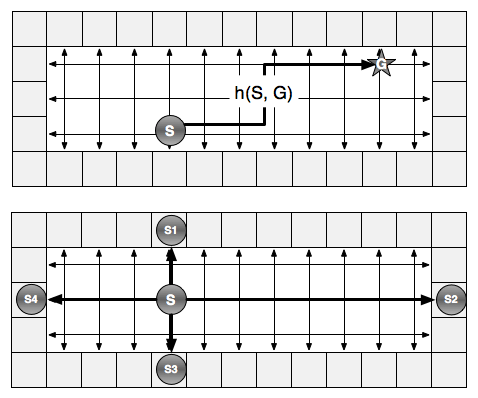
\includegraphics[scale=0.50, trim = 10mm 10mm 10mm 0mm]{diagrams/roomtraversal.png}
       \end{center}
	\vspace{-3pt}
       \caption{The three cases which must be considered in order to prove that 
			optimal traversal of an empty room is possible using only nodes from the perimeter.
			Dashed lines represent macro successors and solid lines represent segments of optimal
			paths that are eventually found}
       \label{fig-ohacontrast}
	\vspace{-15pt}
\end{figure}

\begin{figure*}[htbp]
	\label{fig-oha_contrast}
	\vspace{-4pt}
       \begin{center}
           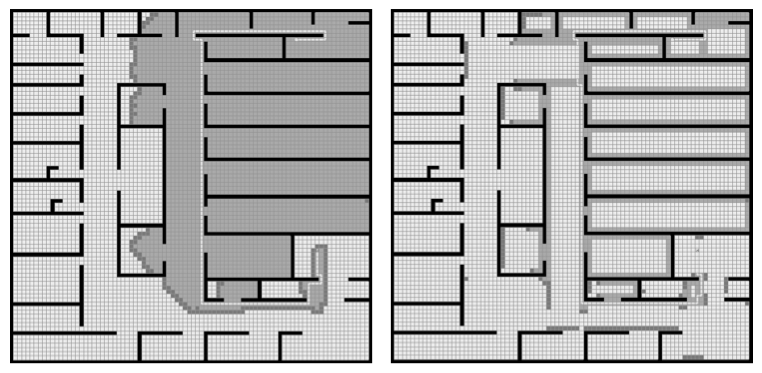
\includegraphics[scale=0.50, trim = 10mm 10mm 10mm 0mm]{diagrams/oha_contrast.png}
       \end{center}
	\vspace{-3pt}
       \caption{\textbf{(a)} A* solving a problem on a typical ($86\times88$) game map. 
Expanded nodes are marked light grey while nodes at the frontier of the search are dark grey.
\textbf{(b)} OHA* solving the same problem. A number of large rooms have been identified (not
all shown) and the algorithm only considers nodes along their perimeter.}
       \label{fig-ohacontrast}
	\vspace{-15pt}
\end{figure*}


\begin{theorem}
OHA* is optimal. 
\end{theorem}
\begin{proof}
To prove this claim we have to show that for every optimal length path $\pi^*(m, n)$ 
on a 4-connected grid map, which starts at node $m$ and terminates at node $n$, 
there exists an equivalent length path $\pi^{*'}(m, n)$ that mentions only nodes from the
perimeter of $R$.
The proof is almost immediate following Lemma \ref{thm-roomtraversal}. 
We will show it is true using an structural proof by induction on the length
of $\pi^{*'}(m, n)$.
\par
For the basis case, suppose node $m$ and $n$ are in the same room $R$.
In this case the optimal $g$-values of $m$ and $n$ are given by:
$$g^*(m) = 0$$
$$ g^*(n) =  \sum_{i = m}^{p(n)}c(k_{i}, k_{i+1})$$ 

where $p(n)$ is the node that precedes $n$ on the optimal path and $c$ is the cost of 
an edge connecting nodes $k_{i}$ and $k_{i+1}$ which appear in sequence along the optimal path 
and are both ancestors of $n$.
We construct $\pi'(m, n)$ by way of Lemma \ref{thm-roomtraversal}, 
which states that we can use the heuristic function $h_{M}$ to directly generate $m$ as a 
macro successor of $n$ if both are in the same room.
Thus we have:

$$ g^{*'}(m) = 0 $$
$$ g^{*'}(n) = h_{M}(m, n)$$

To see that these are equivalent we may restate $g^*(n)$ as:
$$g^*(n) = |x_{m} - x_{n}| + |y_{m} - y_{n}| = h_{M}(m, n)$$

where $x_{m}, y_{m}$ are the coordinates of node $m$ on the map and $x_{n}, y_{n}$ are
the coordinates of node $n$.
We can calculate $g(n)$ in this fashion only because $\pi^*(m,n)$ is optimal and $R$ is
obstacle free which eliminates the possibility that the optimal path contains
 switch-backs (segments where the path doubles back on itself).
Thus $g^{*}(m) = g^{*'}(m)$.
\par
For the inductive case we must show that the same analysis which was true for the basis case
is also true for any segment of the optimal path running through some room $R$. 
Lemma \ref{thm-roomtraversal} gives just such an analysis.
Since every segment of $\pi^{*}(m, n)$ has a corresponding segment in $\pi^{*'}(m, n)$ of equivalent
length it must be that $g^*(n) = g^{*'}(n)$ and $g^*(m) = g^{*'}(m)$.
\end{proof}

To highlight how well OHA* can work in practice consider the example game map in Figure 
\ref{fig-oha_contrast}. 
The topography of this map is typical of what one might expect in a modern role-playing game
\footnote{Infact, most video game maps tend to be somewhat bigger than our example but for demonstration 
purposes it is quite sufficient.};
there are many rooms and corridors and many entrances to connect them.
Figure \ref{fig-oha_contrast}(a) shows A* solving a typical problem on this map. 
In this case obtaining the optimal solution required expanding almost half the nodes in the state space.
Figure \ref{fig-oha_contrast}(b) shows the same problem being solved by OHA*.
We were able to prune away large sections of the map by taking advantage of the fact that
such nodes never need to be expanded in order to retain optimality.
In this case OHA* expands less than $\frac{1}{3}$ of the area explored by A* and returns
a solution 4 times faster.

